\documentclass{beamer}
\usepackage[utf8]{inputenc}
\usepackage[frenchb]{babel}
\usepackage[T1]{fontenc}
\usepackage{graphics}
\usepackage{framed}
\usepackage{graphicx}
\usetheme{Warsaw}

\title[Support pour Verificarlo]{Support de MPI/OpenMP et de la vectorisation dans Verificarlo}
\subtitle{Master Calcul Haute Performance et Simulation}

\author[Hery, Ali, Nicolas]{Hery ANDRIANANTENAINA \\ Ali LAKBAL \\ Nicolas BOUTON}

\institute{\textbf{Encadrant:} Eric PETIT}

\date{Année 2020-2021}

\begin{document}

\maketitle

\begin{frame}{Verificarlo}

  \begin{itemize}
  \item Compilateur: \textbf{ Clang et llvm} 
  \item Domaine d'utilisation: \textbf{ Instrumentation des opérations flottantes}
  \end{itemize}
  
  \textbf{1. Vectorisation dans le calcul scientifique}
  
\end{frame}

\begin{frame}{Benchmark}

  \begin{block}{Backends utilisés}
    \begin{itemize}
    \item ieee
    \item vprec
    \end{itemize}
  \end{block}

  \begin{block}{Language}
    Language C
  \end{block}
  
  \begin{block}{Opérations testés:}
    \begin{itemize}
    \item r += v
    \item r -= v
    \item r *= v
    \item r /= v
    \end{itemize}
  \end{block}

\end{frame}

\begin{frame}{Paramètre}

  \begin{block}{Paramètre de la machine de test}
    \begin{itemize}
    \item OS: Linux Manjaro avec i3
    \item Jeu d'instruction: SSE

    \end{itemize}
  \end{block}

  \begin{block}{Paramètre du Benchmark}
    \begin{itemize}
    \item Programme assigné au dernier coeur
    \item Test les zones mémoires: caches + DRAM
    \item Nombres d'itérations: 1000
    \item Dérivation standard faible
    \end{itemize}
  \end{block}

\end{frame}

\begin{frame}{Backend ieee}

  \begin{center}
    \begin{figure}
      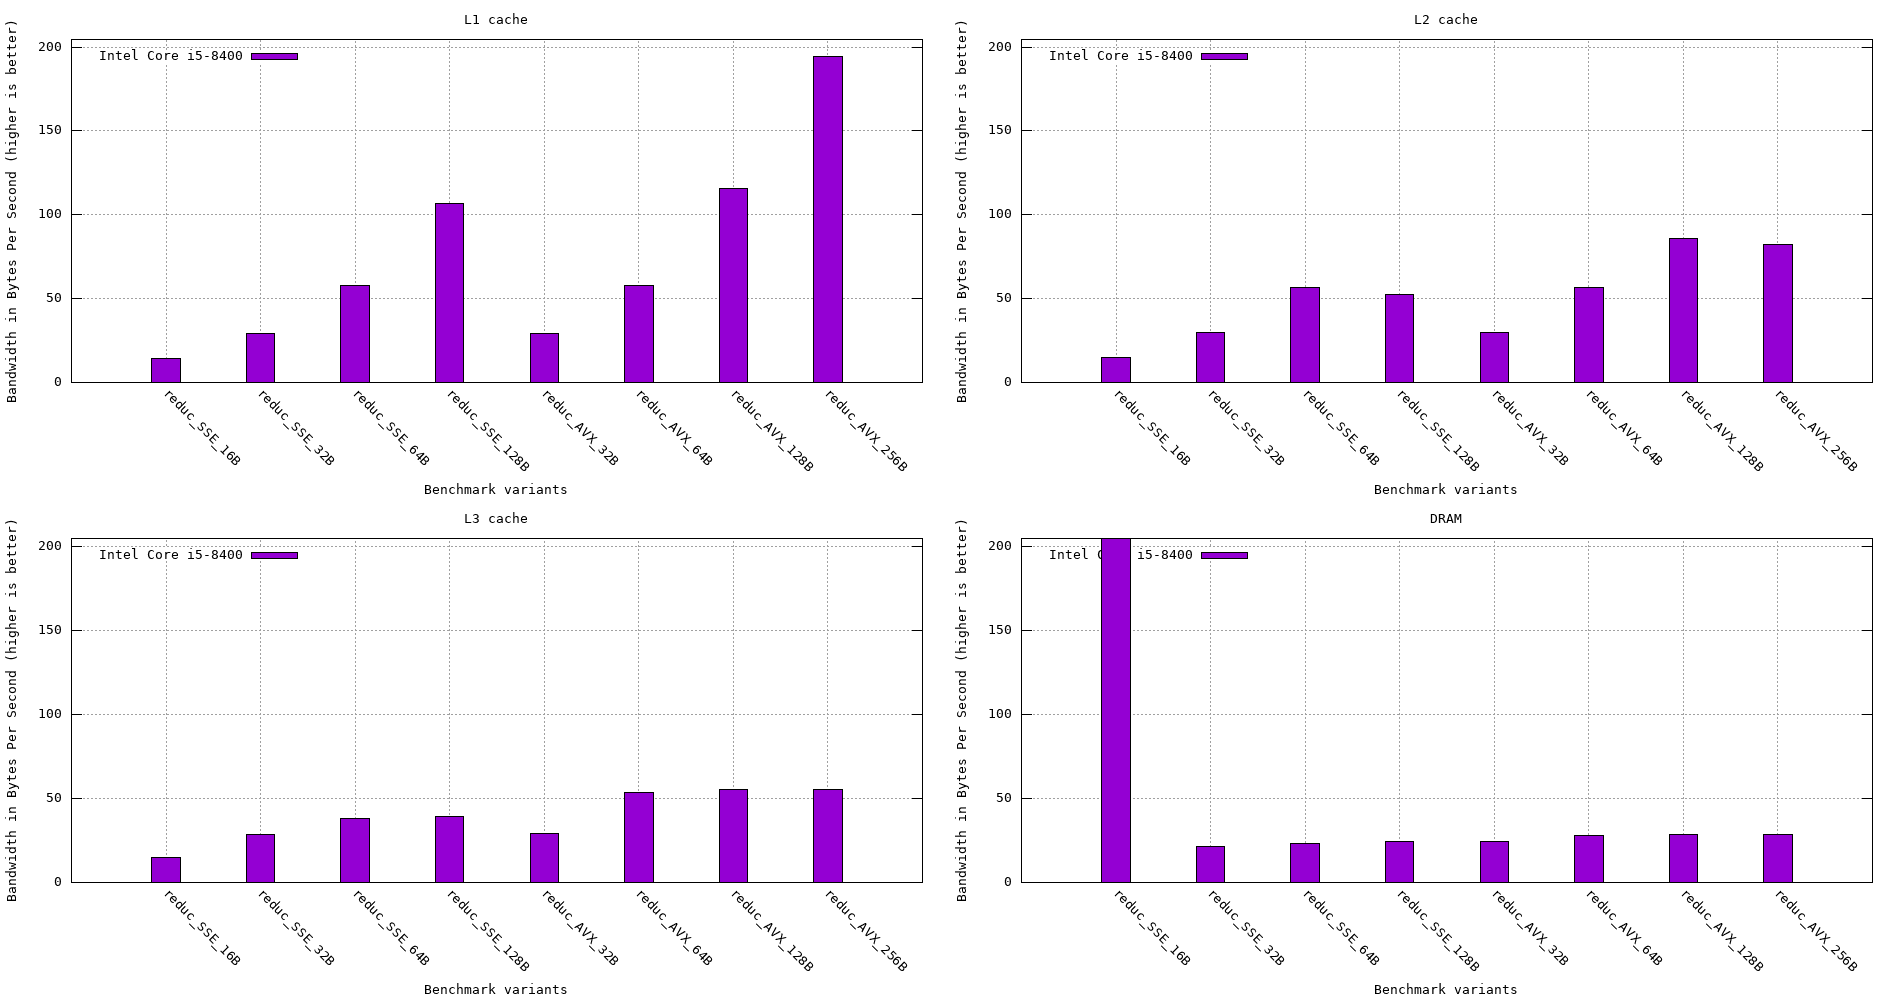
\includegraphics[scale=0.2]{../ressources/ieee_bw.png}
      \caption{\label{fig:backend_ieee}Benchmark pour le backend ieee}
    \end{figure}
  \end{center}
  
\end{frame}

\begin{frame}{Backend vprec}

  \begin{center}
    \begin{figure}
      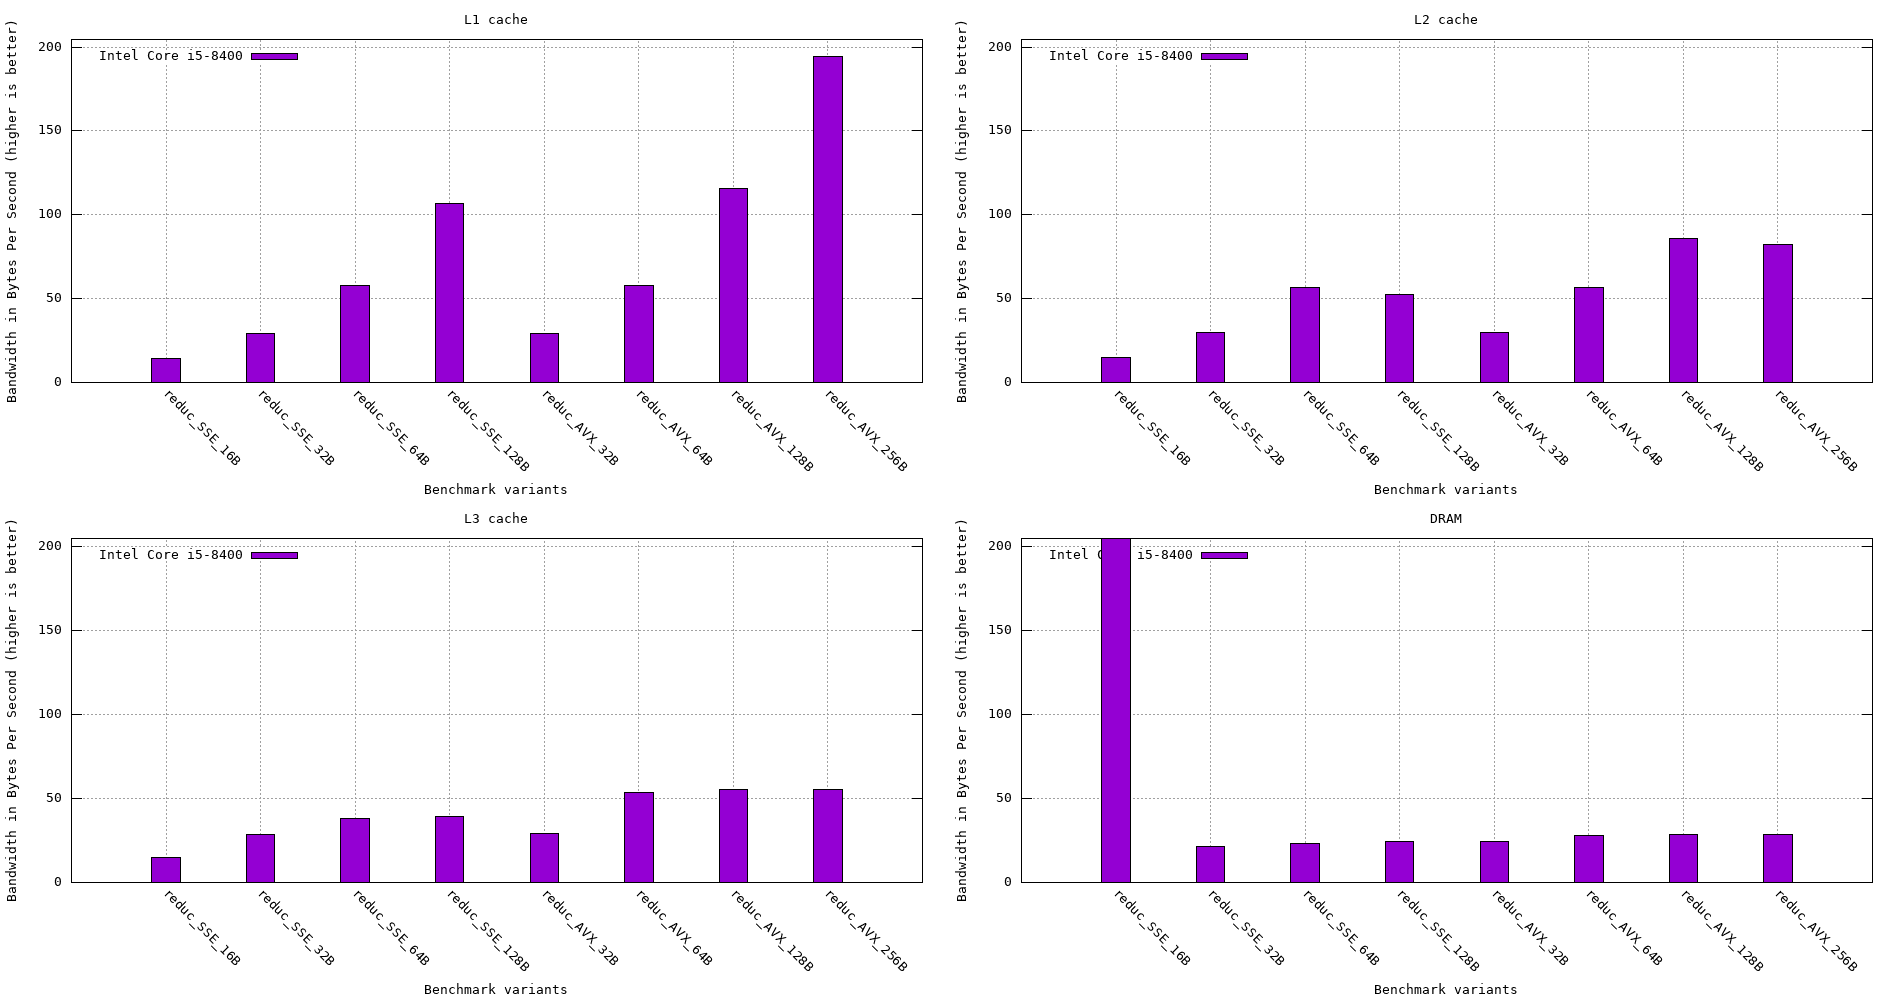
\includegraphics[scale=0.2]{../ressources/vprec_bw.png}
      \caption{\label{fig:backend_vprec}Benchmark pour le backend vprec}
    \end{figure}
  \end{center}
  
\end{frame}

\end{document}
